\chapter{Temperature validation and change for the RegCM simulations}  \label{appendix_tas}
The two RegCM simulations described in \cref{sec:experiments} are here briefly analysed for what concerns temperature.
In the reference period, the comparison is performed against the UDEL\citep{Willmott2001}, CRU\citep{Harris2014} and E-OBS \citep{Haylock2008} datasets.
\Cref{fig:valid_rcm_tas_ac} show the annual cycle of the two simulations, compared with that of observations.
In both cases, biases with observations are relatively minor, with the model being slightly too cold in winter in all regions, and slightly too hot (cold) in the North (South) in summer.\\
A spatial comparison is presented in \cref{fig:valid_rcm_tas_mean}. Average seasonal temperatures are significantly easier for the model to simulate compared to precipitation, and all major features are well reproduced.
An overestimation of summer temperatures in the Po plain is found, together with a general underestimation of high elevation temperatures in winter.
Uncertainties between observations are also greatly reduced for this variable, with all the three dataset showing similar spatial patterns and values.
\begin{figure}
    \centering
    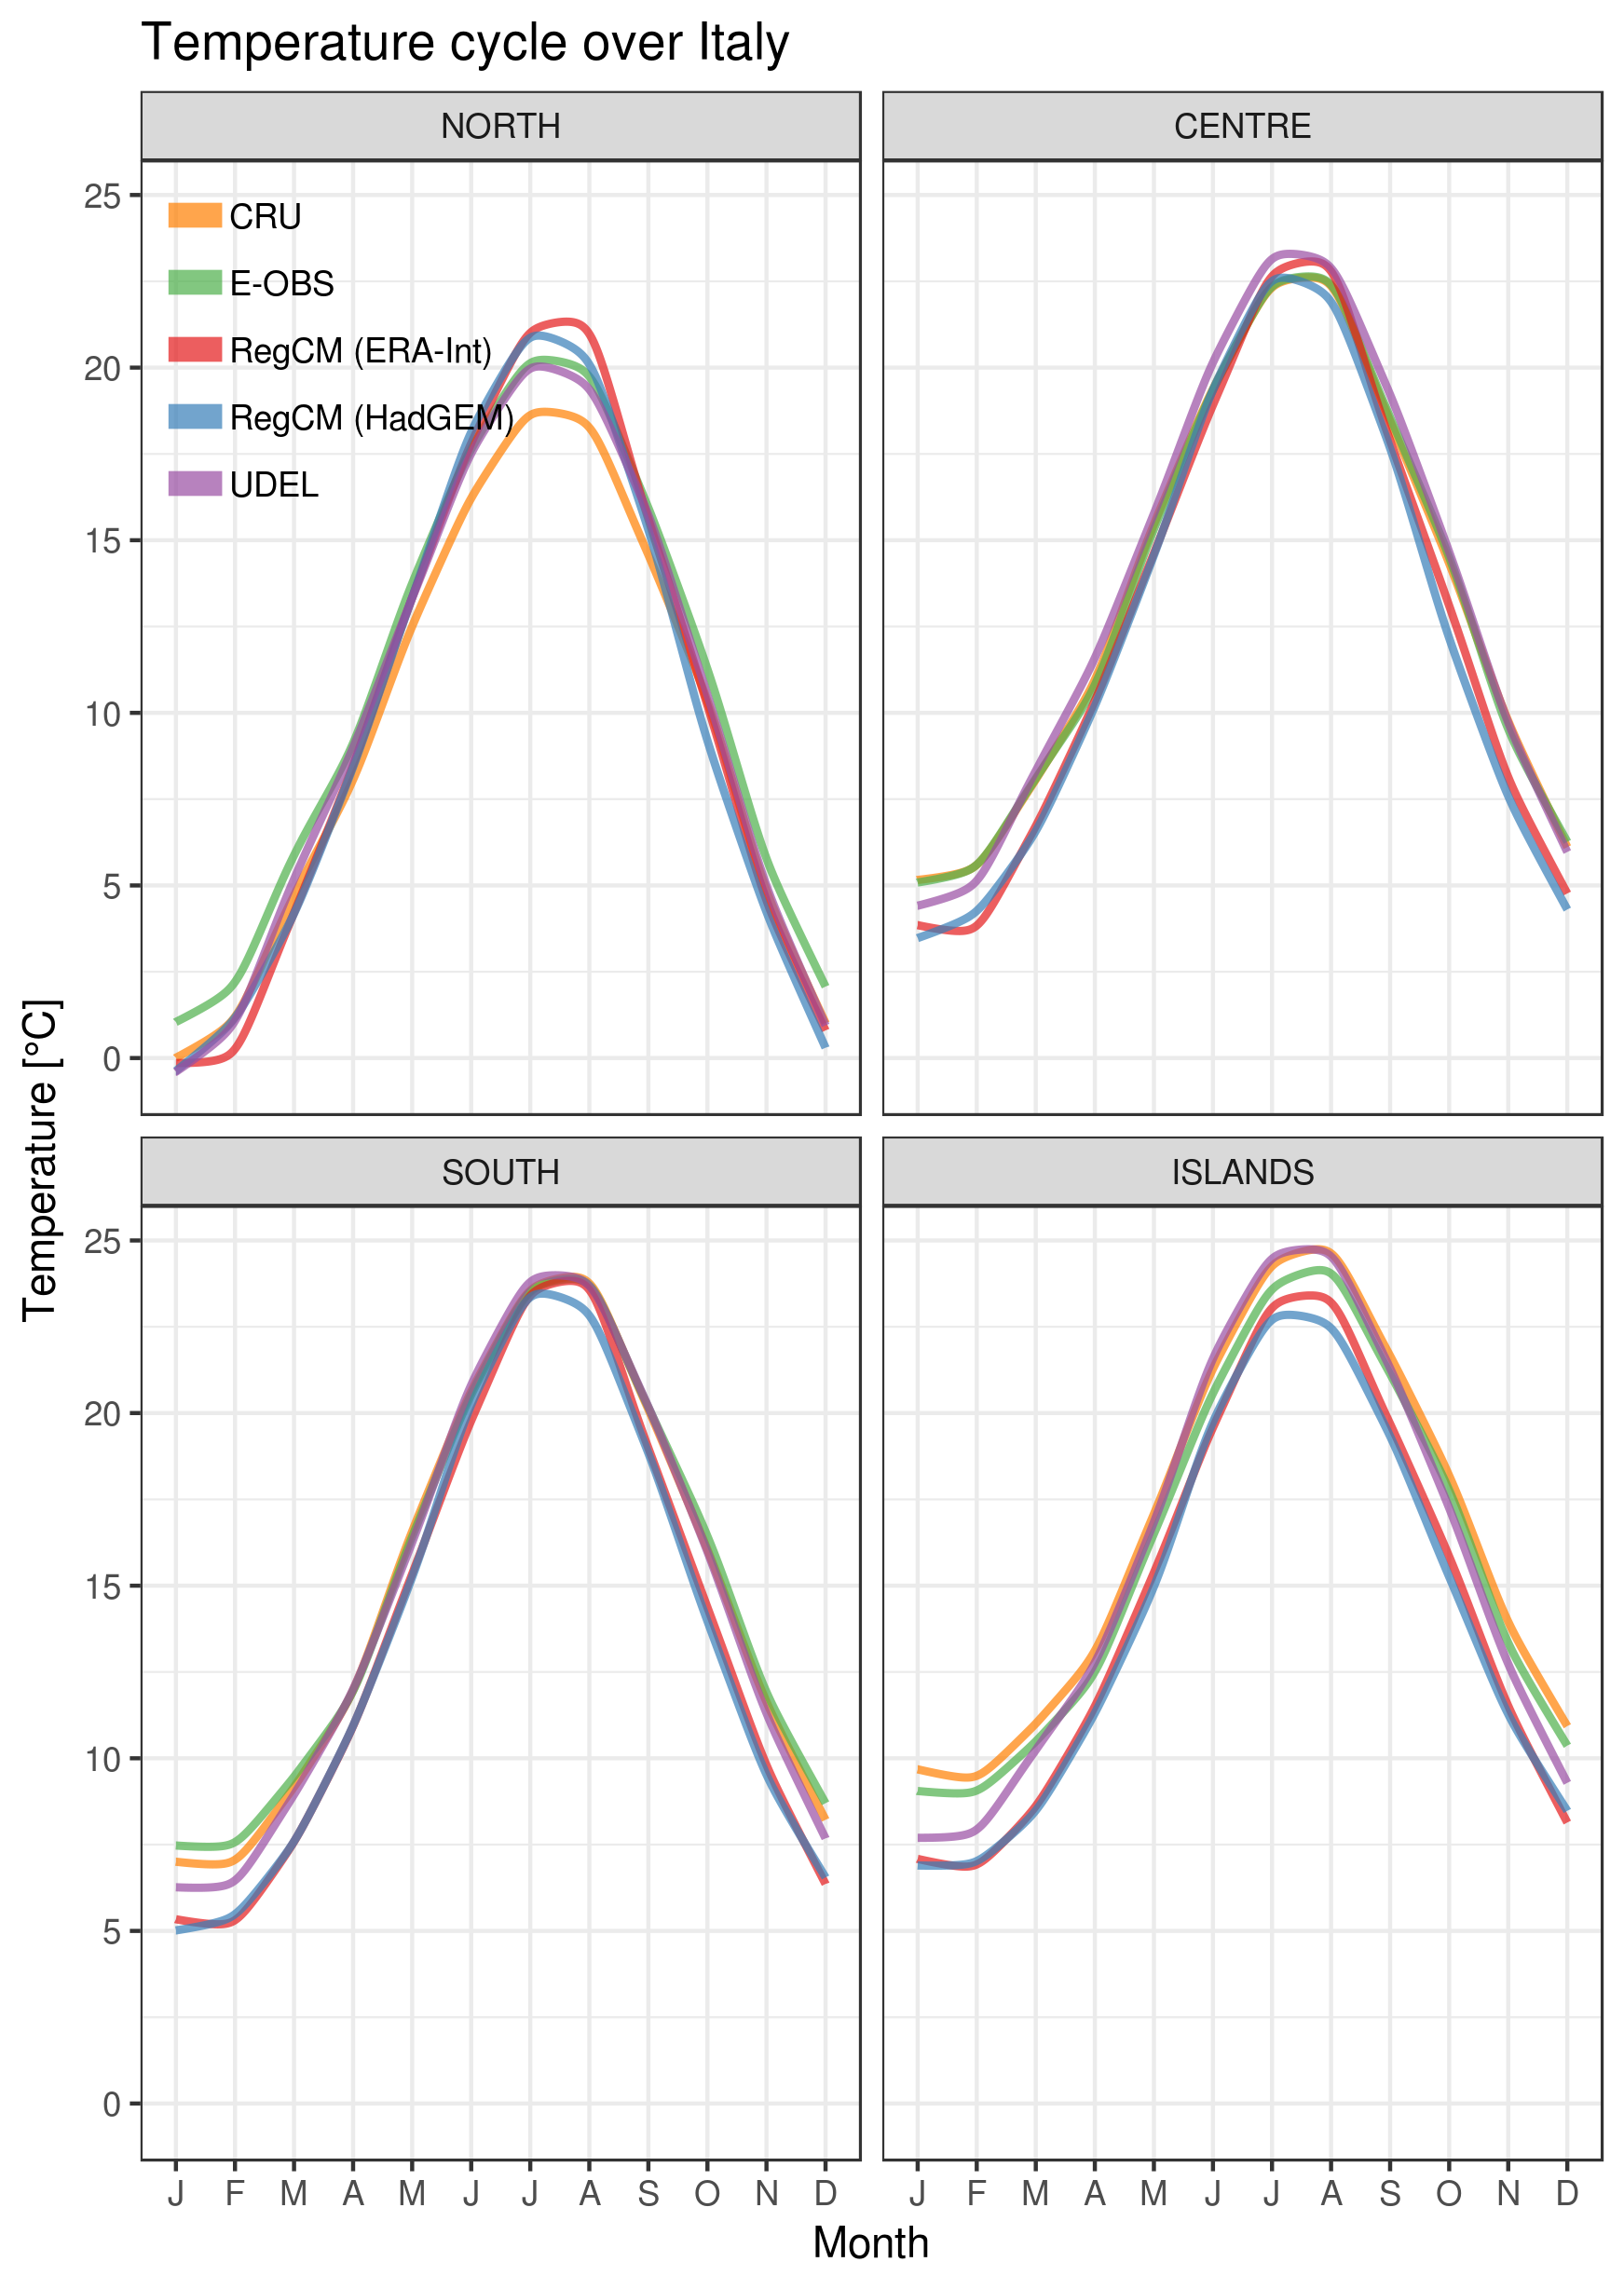
\includegraphics[width=0.7\textwidth]{figures/valid_rcm/tas/ac}
    \decoRule
    \caption[Validation of temperature annual cycle]{
        Annual cycle of temperature as reproduced by observations and models (\cref{sec:experiments}). The time period for each dataset varies according to availability. The four macroregions selected are the same as in previous evaluations (\cref{sec:uncertainty_pr,sec:validation_itaobs}).
    }\label{fig:valid_rcm_tas_ac}
\end{figure}
\begin{figure}
    \centering
    \includegraphics[width=0.9\textwidth]{figures/valid_rcm/tas/mean}
    \decoRule
    \caption[Validation of average seasonal temperature]{
        Average seasonal temperature for the two climate model simulations (top two rows) and three selected temperature datasets.
    } \label{fig:valid_rcm_tas_mean}
\end{figure}

% \begin{figure}
%     \centering
%     \begin{subfigure}{0.8\textwidth}
%         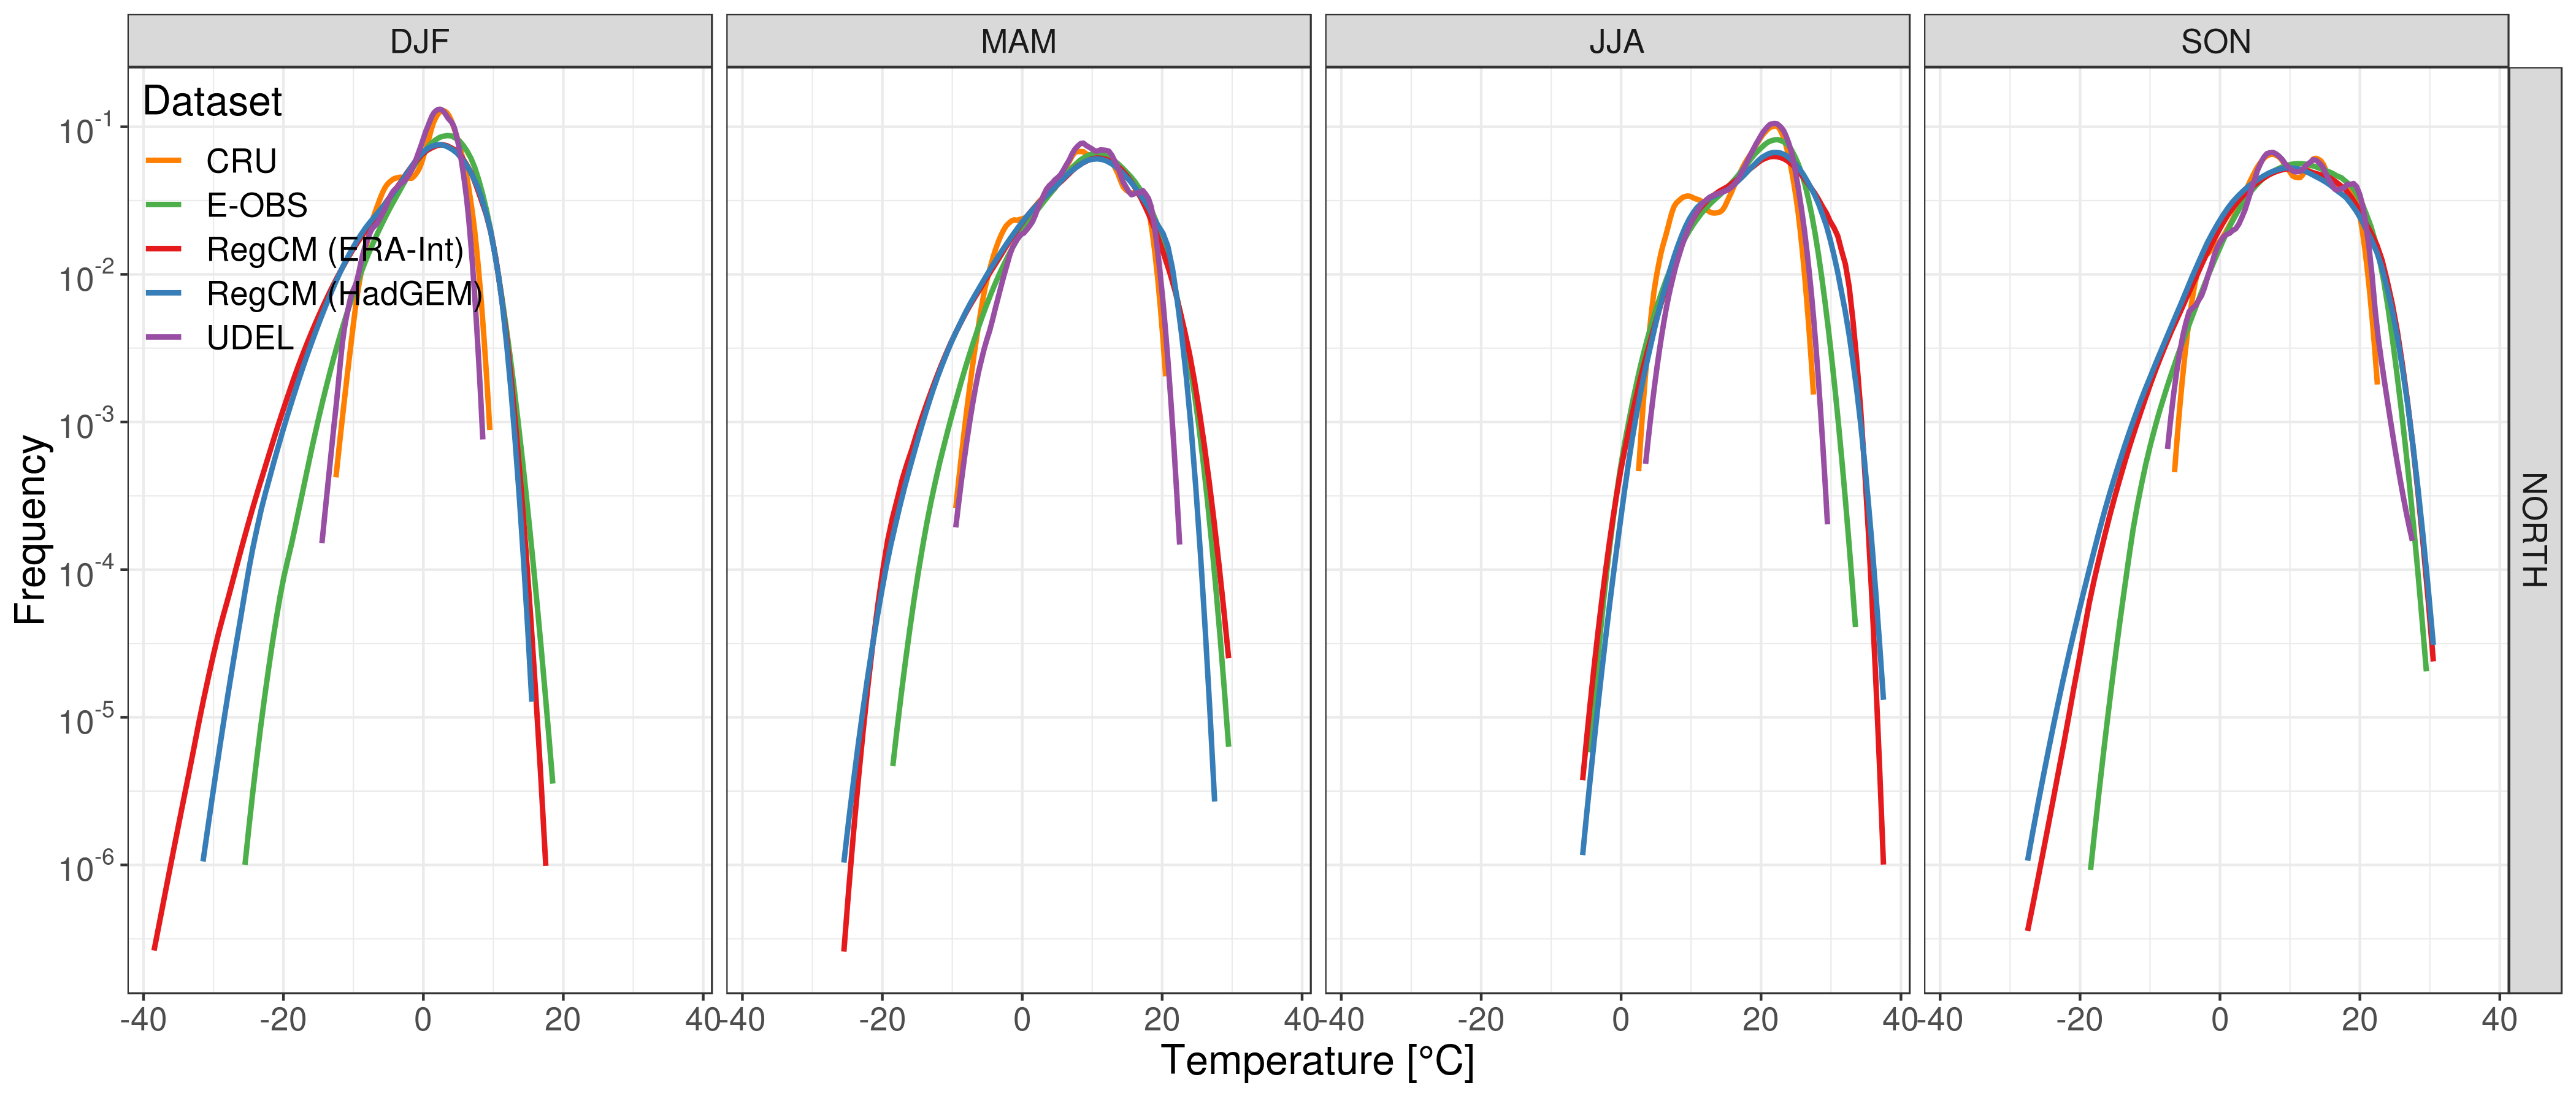
\includegraphics[width=\textwidth]{figures/valid_rcm/tas/pdf_NORTH_lines}
%     \end{subfigure}\\
%     \begin{subfigure}{0.8\textwidth}
%         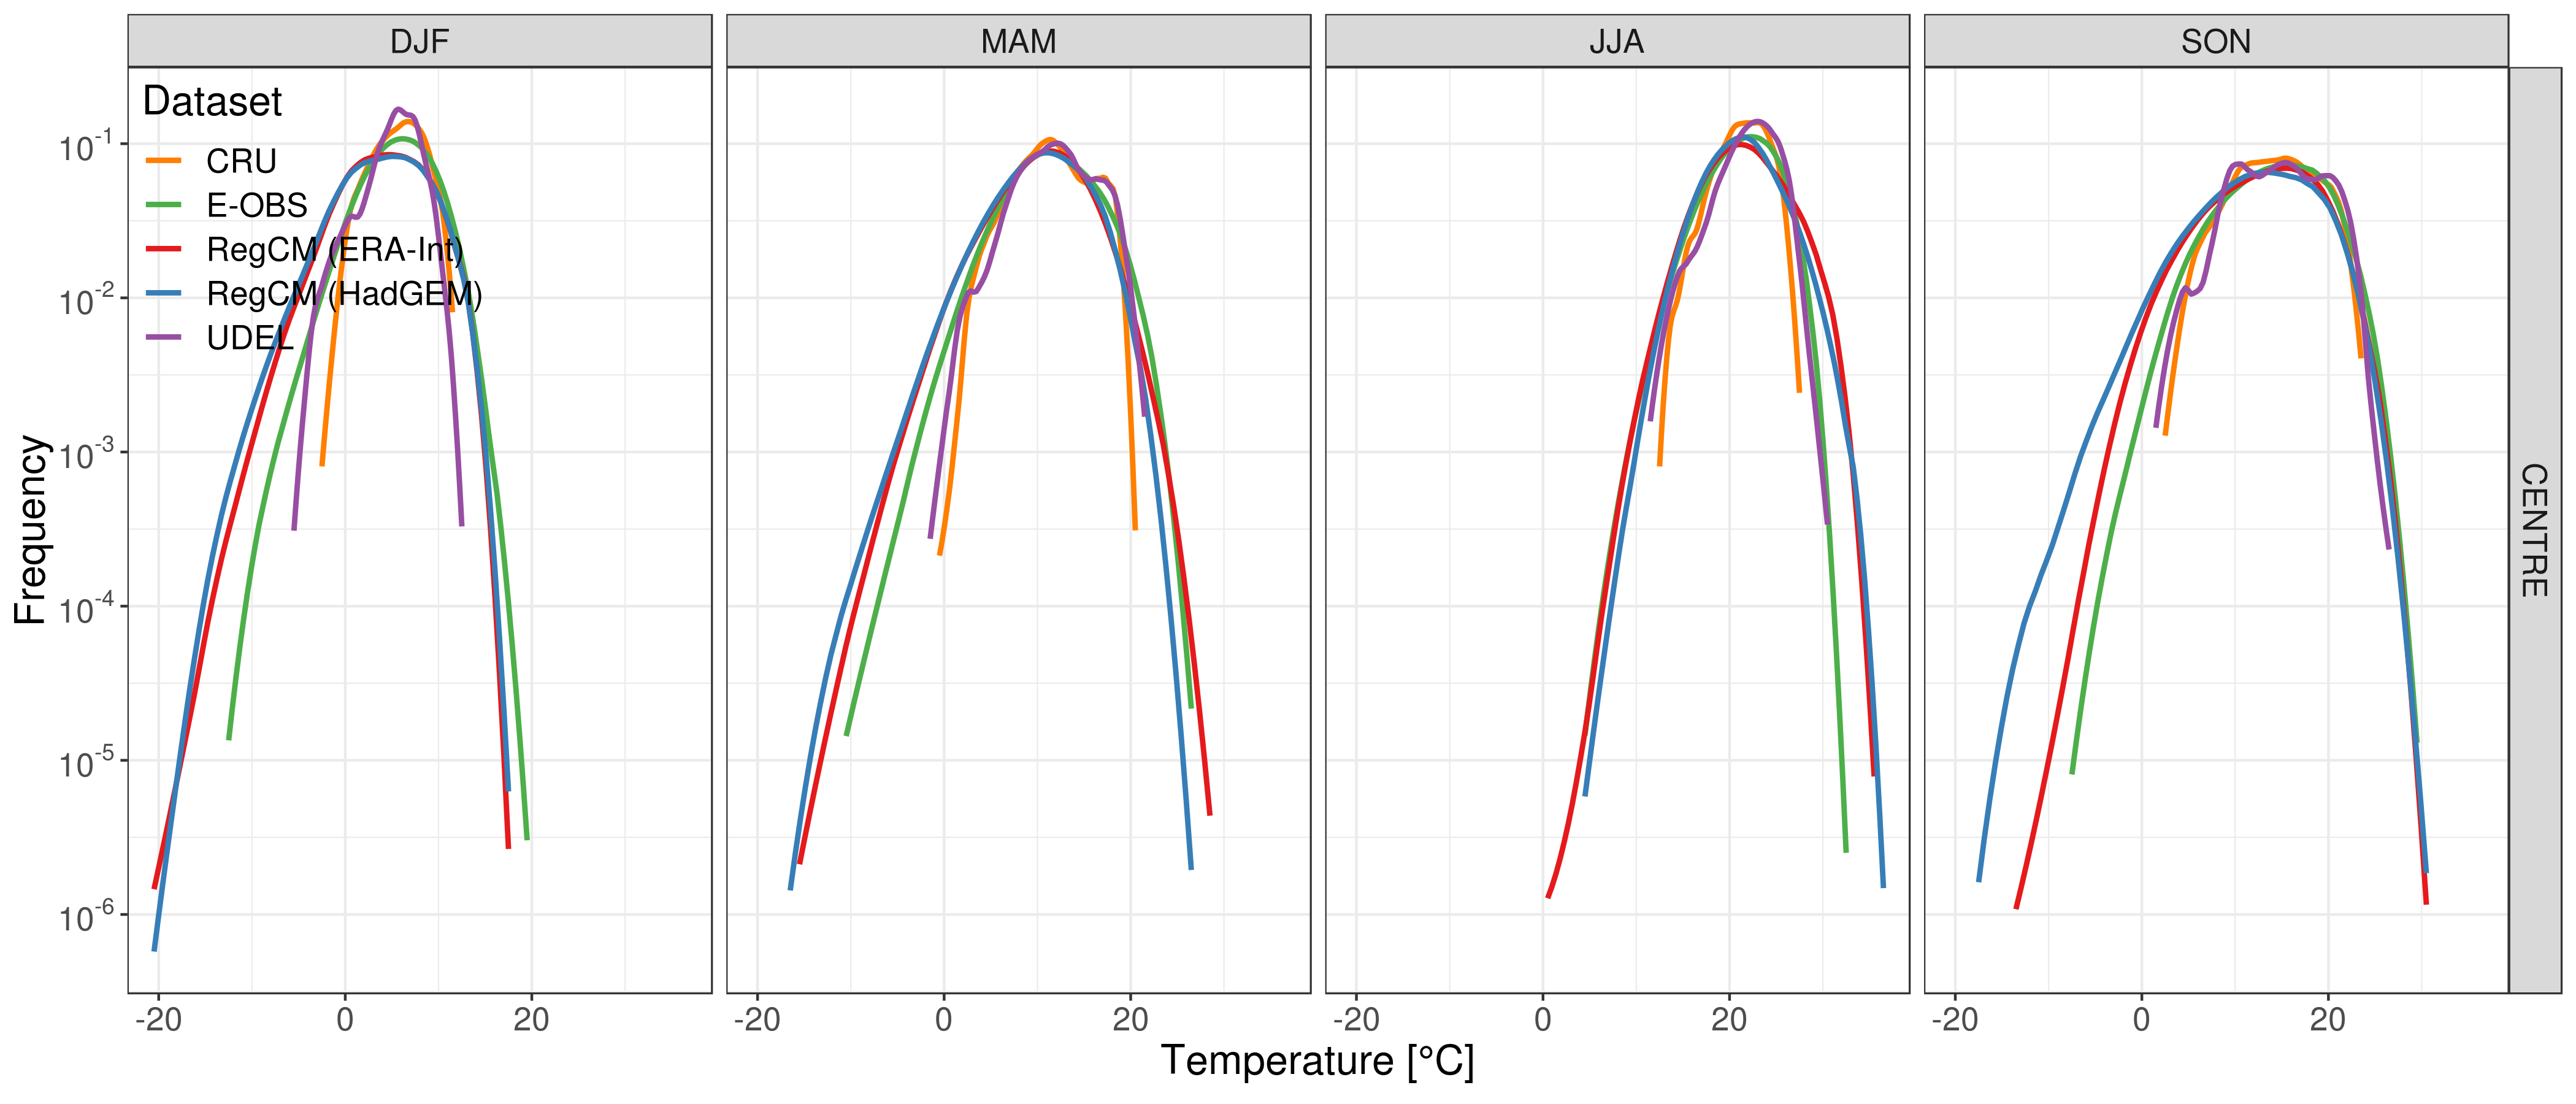
\includegraphics[width=\textwidth]{figures/valid_rcm/tas/pdf_CENTRE_lines}
%     \end{subfigure}\\
%     \begin{subfigure}{0.8\textwidth}
%         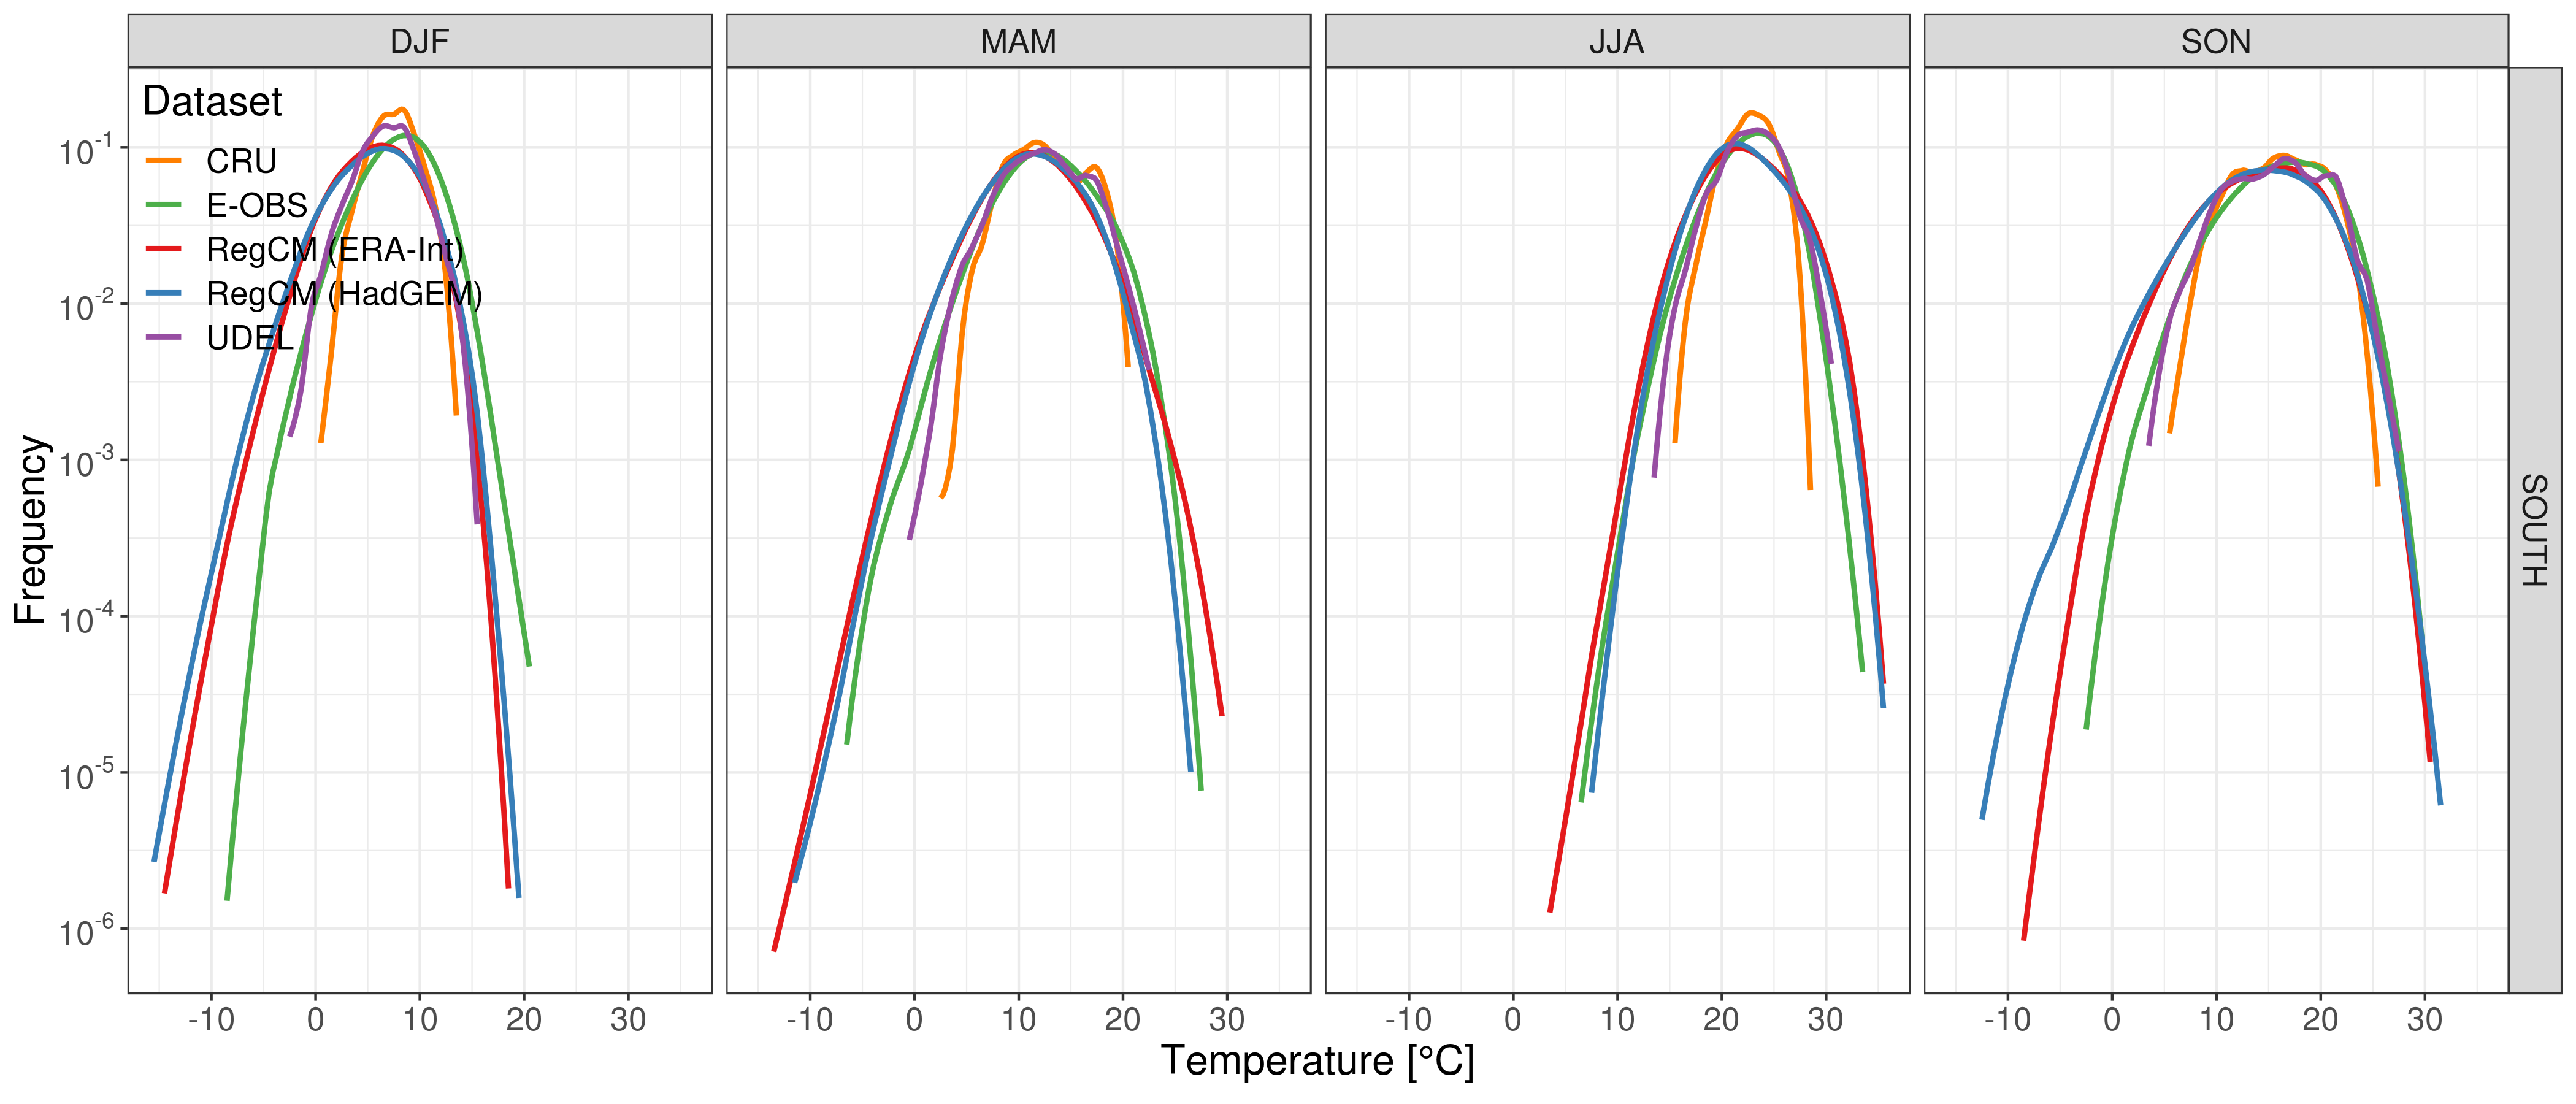
\includegraphics[width=\textwidth]{figures/valid_rcm/tas/pdf_SOUTH_lines}
%     \end{subfigure}\\
%     \begin{subfigure}{0.8\textwidth}
%         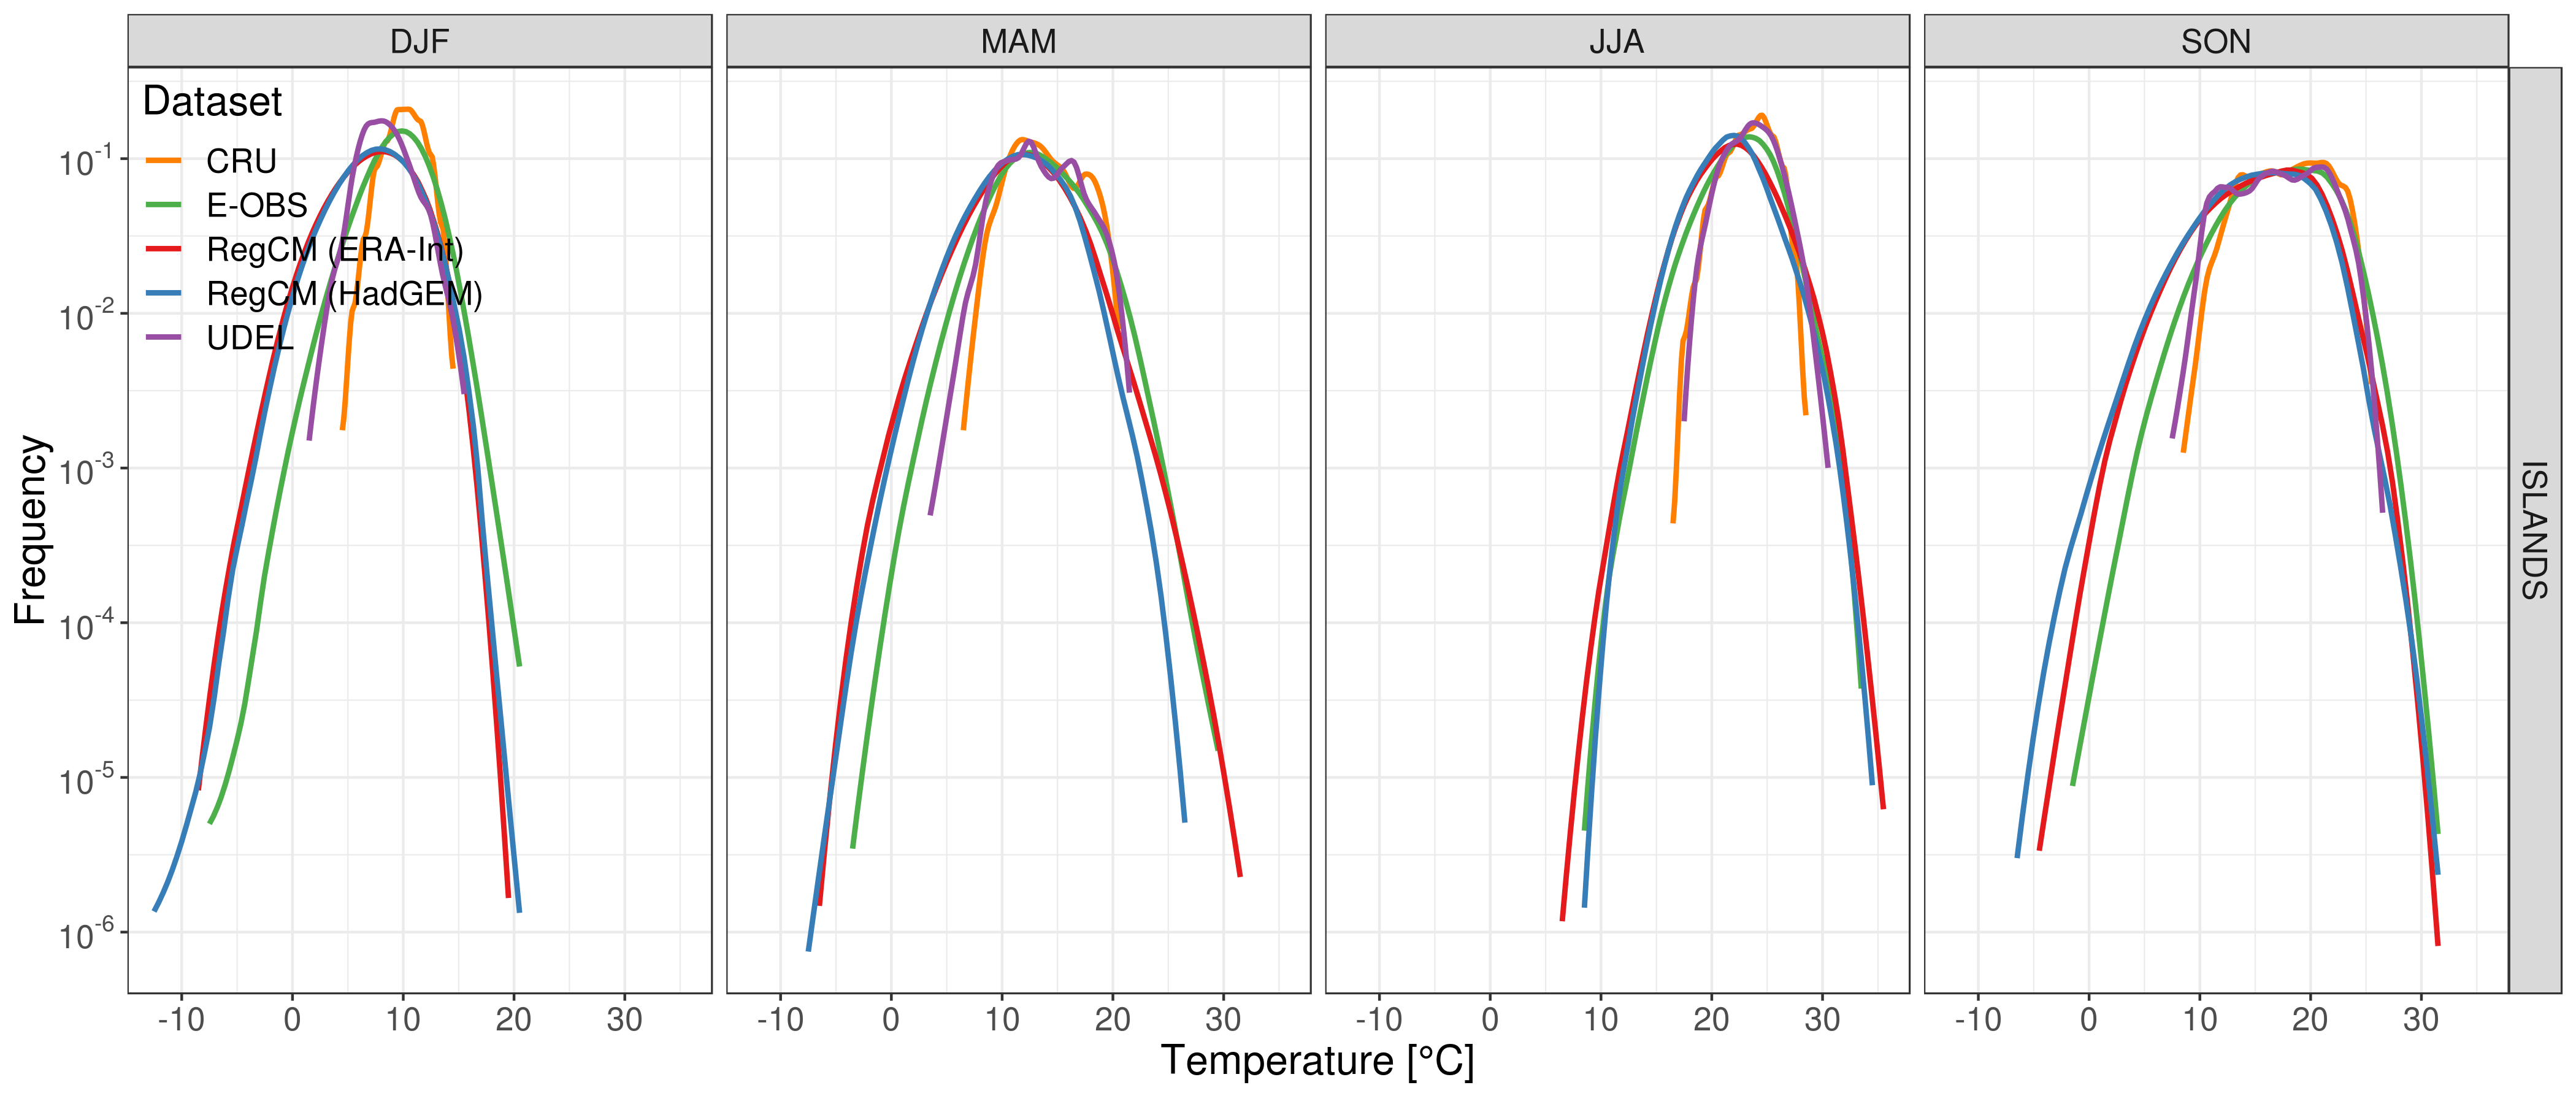
\includegraphics[width=\textwidth]{figures/valid_rcm/tas/pdf_ISLANDS_lines}
%     \end{subfigure}
%     \decoRule
%     \caption[Validation of temperature PDFs]{
%         Daily seasonal temperature Probability Density Functions for the four macroregions.
%     }\label{fig:valid_rcm_tas_pdf}
% \end{figure}

For the RegCM (HadGEM) simulation, future changes in temperature can be reduced to a general increase, pretty uniform across all of the domain.
Land areas warm up slightly more than water surfaces.
The temperature changes range from to \SIrange{3}{7}{\celsius}, with average changes of \SIrange{3.7}{6.2}{\celsius}.
The increase is stronger in summer and weaker in winter.\\
Temperature PDFs (not shown) are also mainly characterised by a uniform, constant increase across all the frequencies, seasons and regions.
This means that extremely cold days generally disappear in the 2070--2099 timeslice, while high temperature events that can be considered extreme in the reference period become much more common by the end of the century: \SI{30}{\celsius} summer days in Sardinia and Sicily, for example, become more than ten times more frequent.

\begin{figure}
    \centering
    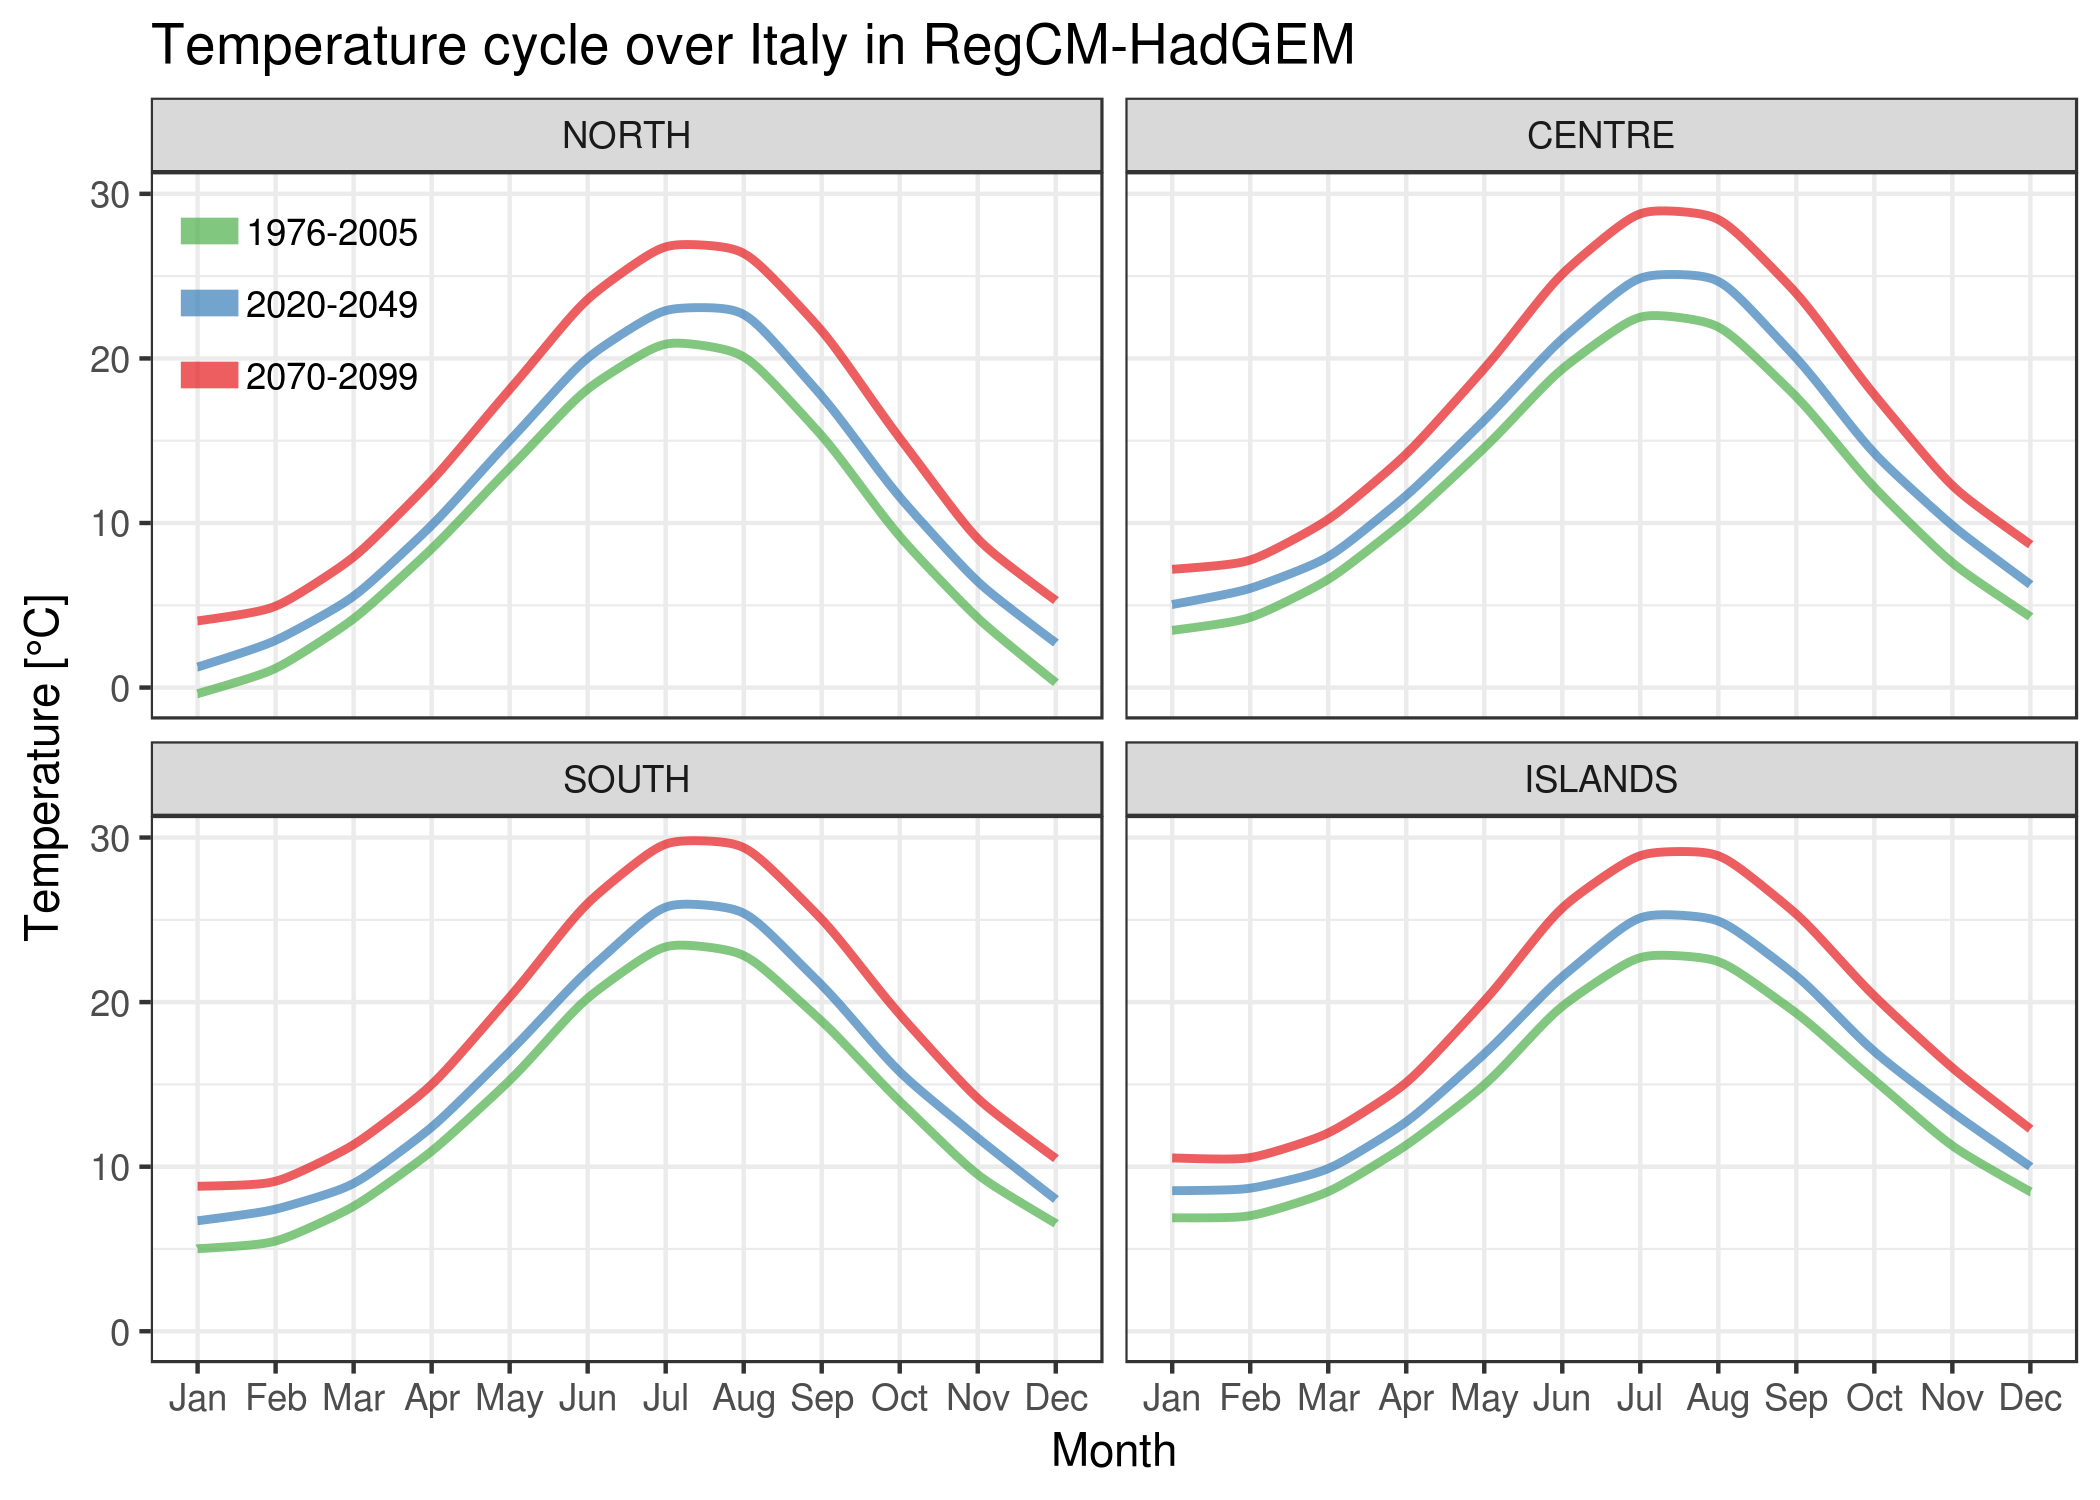
\includegraphics[width=\textwidth]{figures/change_rcm/tas/ac}
    \decoRule
    \caption[Future change in the temperature annual cycle]{
        The temperature annual cycle for the RegCM (HadGEM) simulation in the three timeslices selected, for the four macroregions (see \cref{sec:uncertainty_pr,sec:validation_itaobs}).
    }\label{fig:change_rcm_tas_ac}
\end{figure}
\begin{figure}
    \centering
    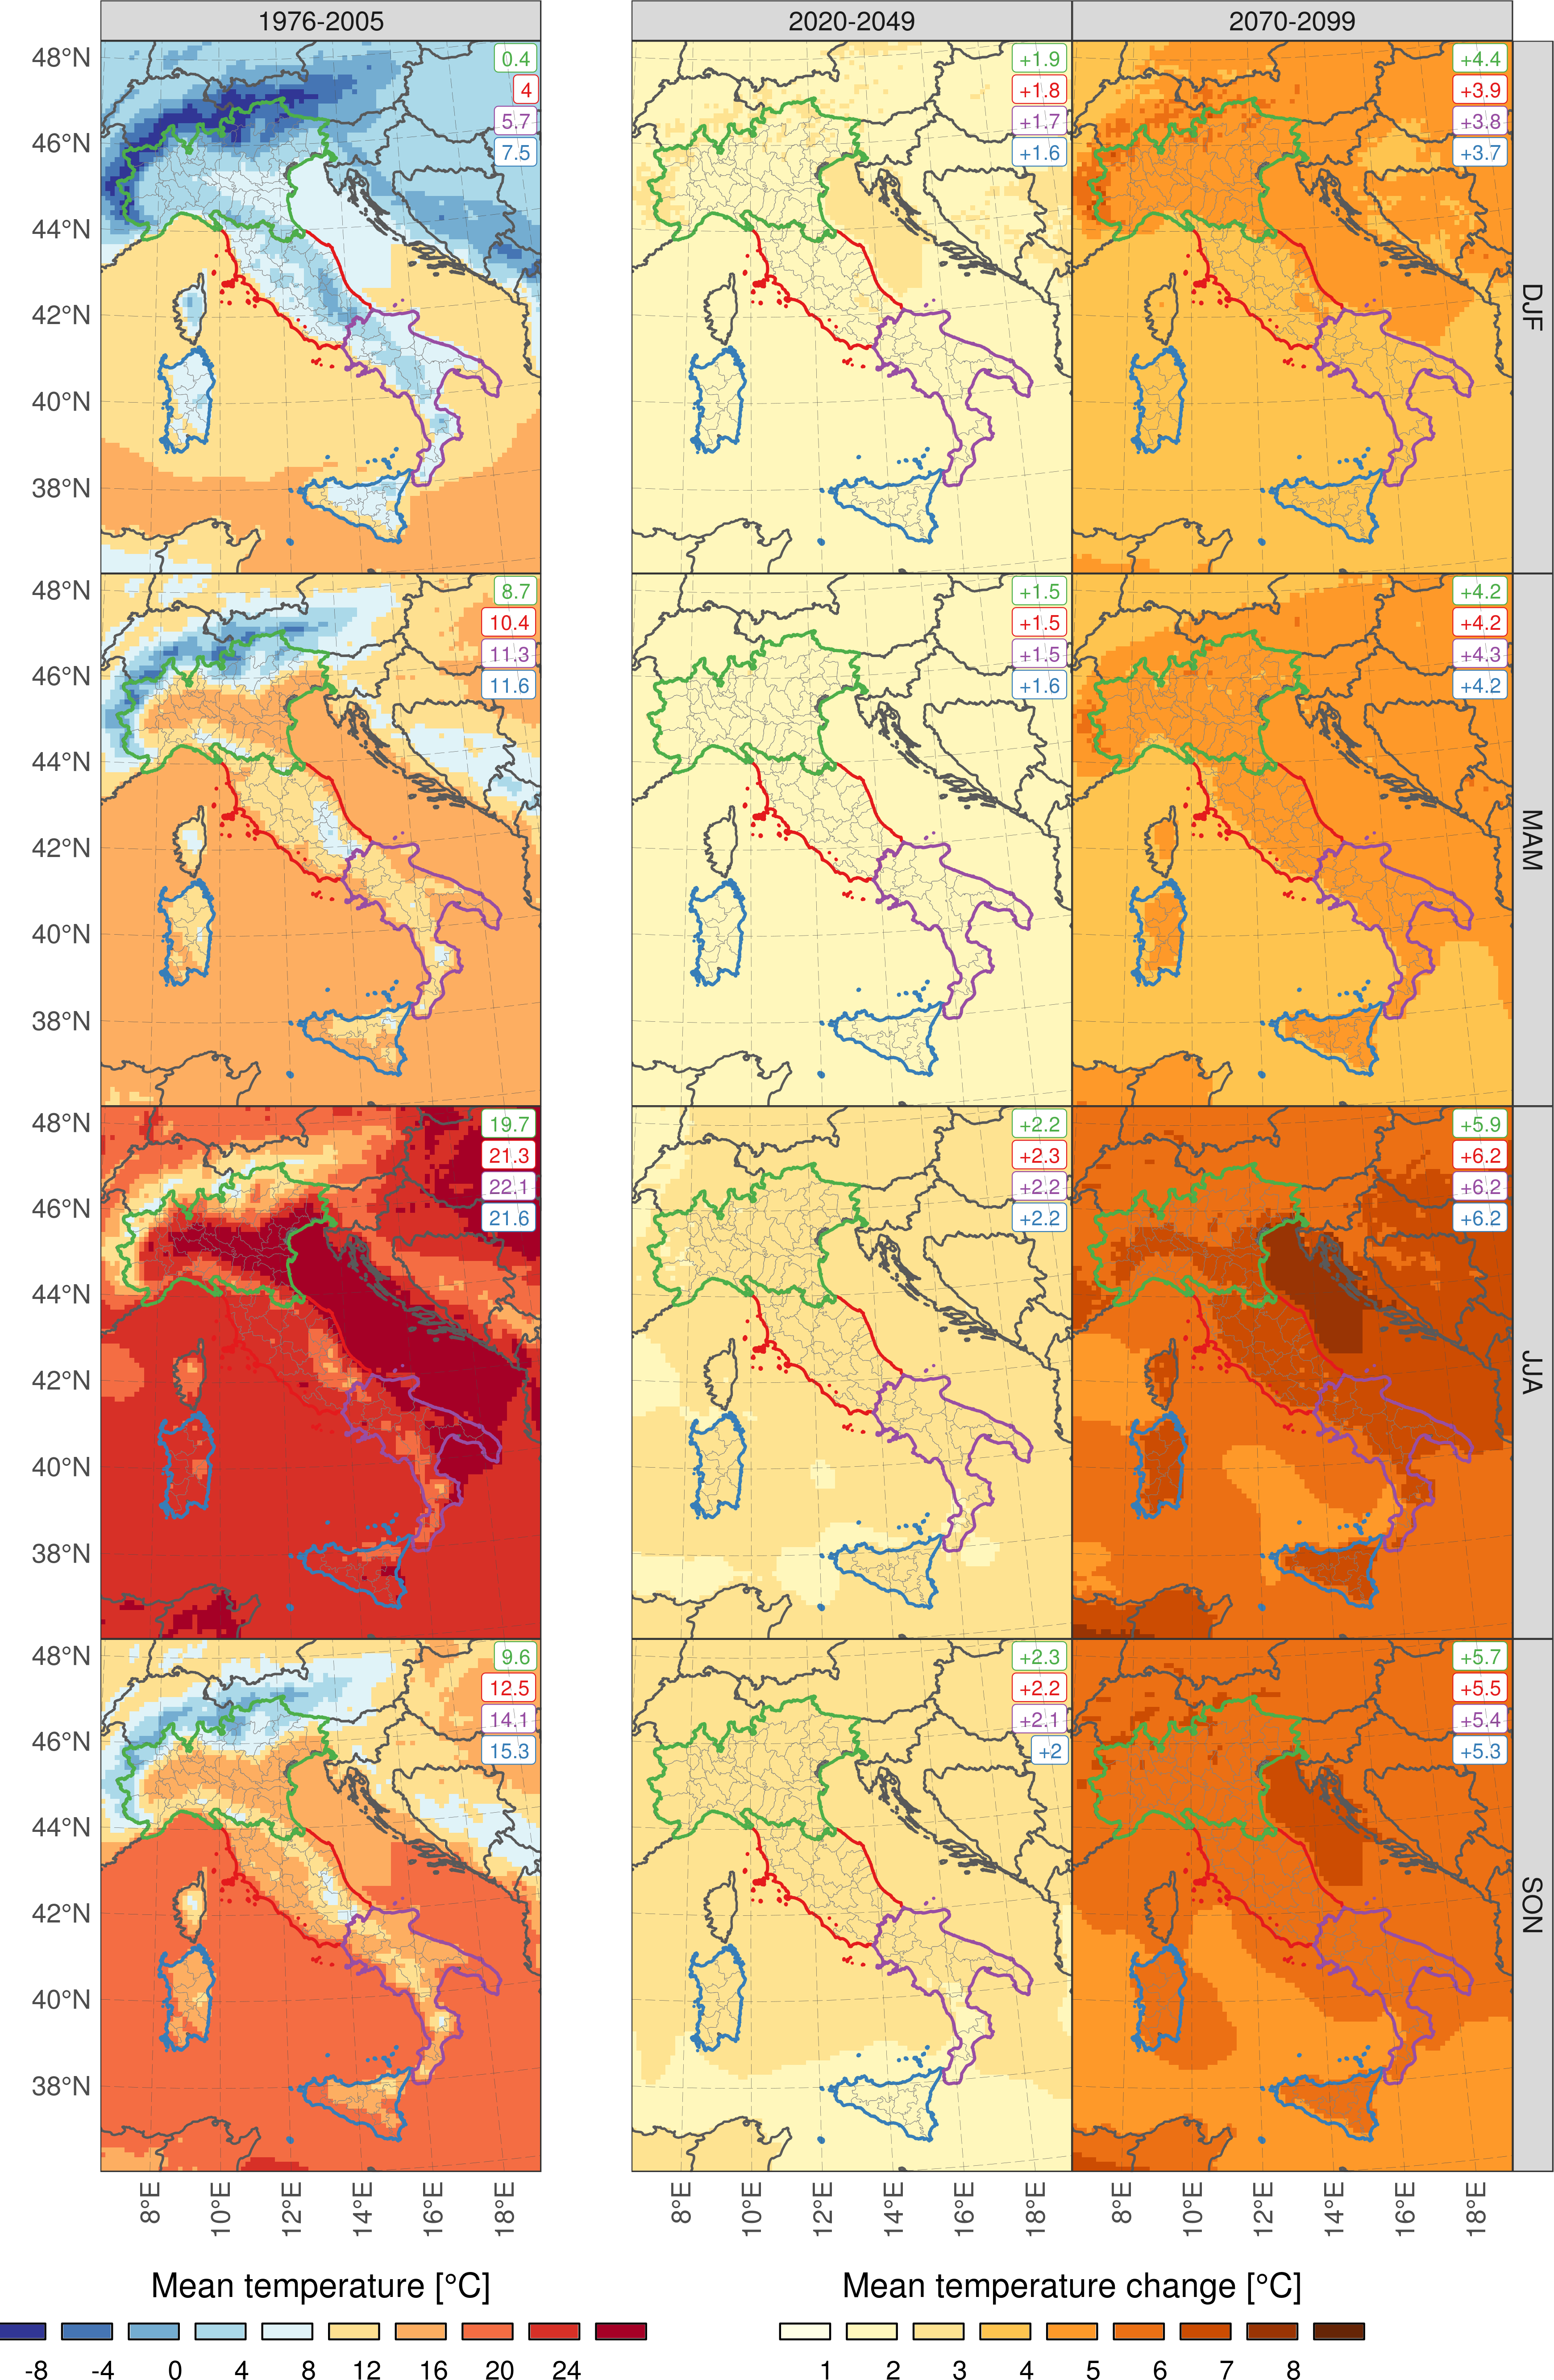
\includegraphics[width=\textwidth]{figures/change_rcm/tas/mean_change_3col}
    \decoRule
    \caption[Future change of the average seasonal temperature]{
        Average seasonal temperature for the RegCM (HadGEM) simulation for the reference period (left column) and change w.r.t. it (centre and right column). The four rows represent seasons. In the top right corner of each map, the colour-coded average for each of the four macroregions is shown.
    } \label{fig:change_rcm_tas_mean}
\end{figure}

\begin{figure}
    \centering
    \begin{subfigure}{0.8\textwidth}
        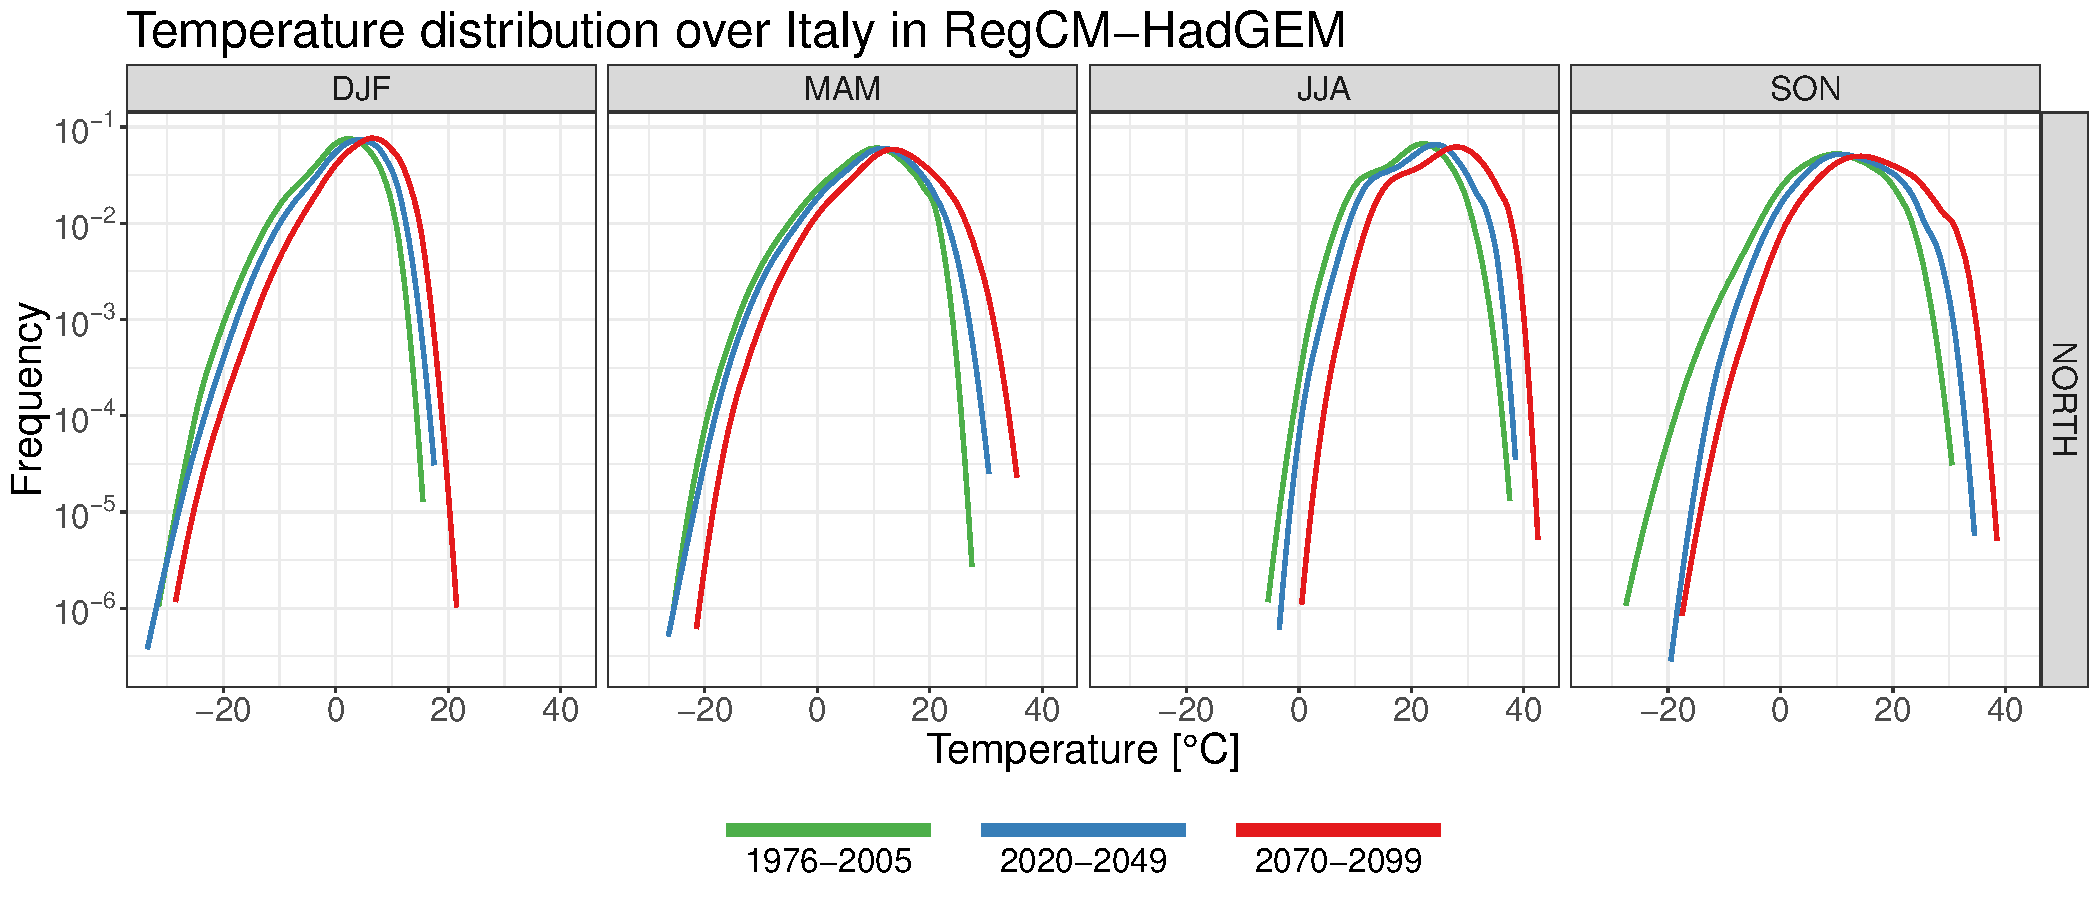
\includegraphics[width=\textwidth]{figures/change_rcm/tas/pdf_NORTH_lines}
    \end{subfigure}\\
    \begin{subfigure}{0.8\textwidth}
        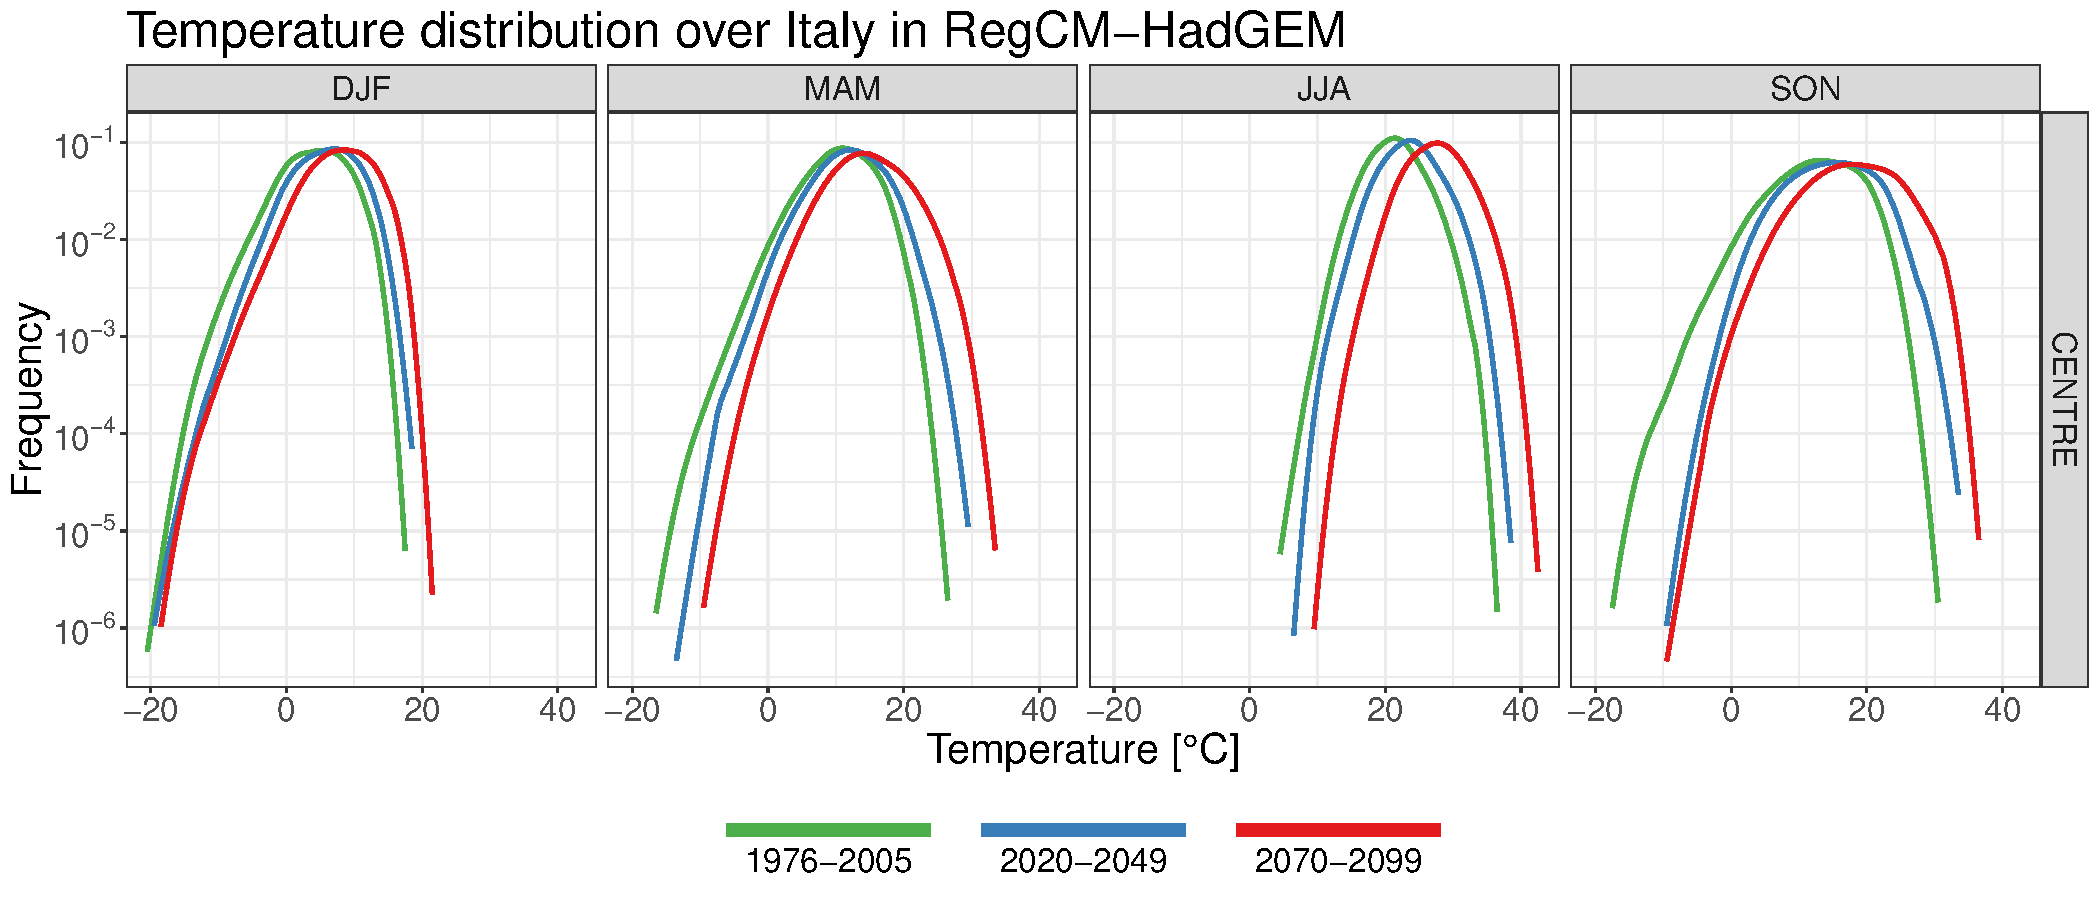
\includegraphics[width=\textwidth]{figures/change_rcm/tas/pdf_CENTRE_lines}
    \end{subfigure}\\
    \begin{subfigure}{0.8\textwidth}
        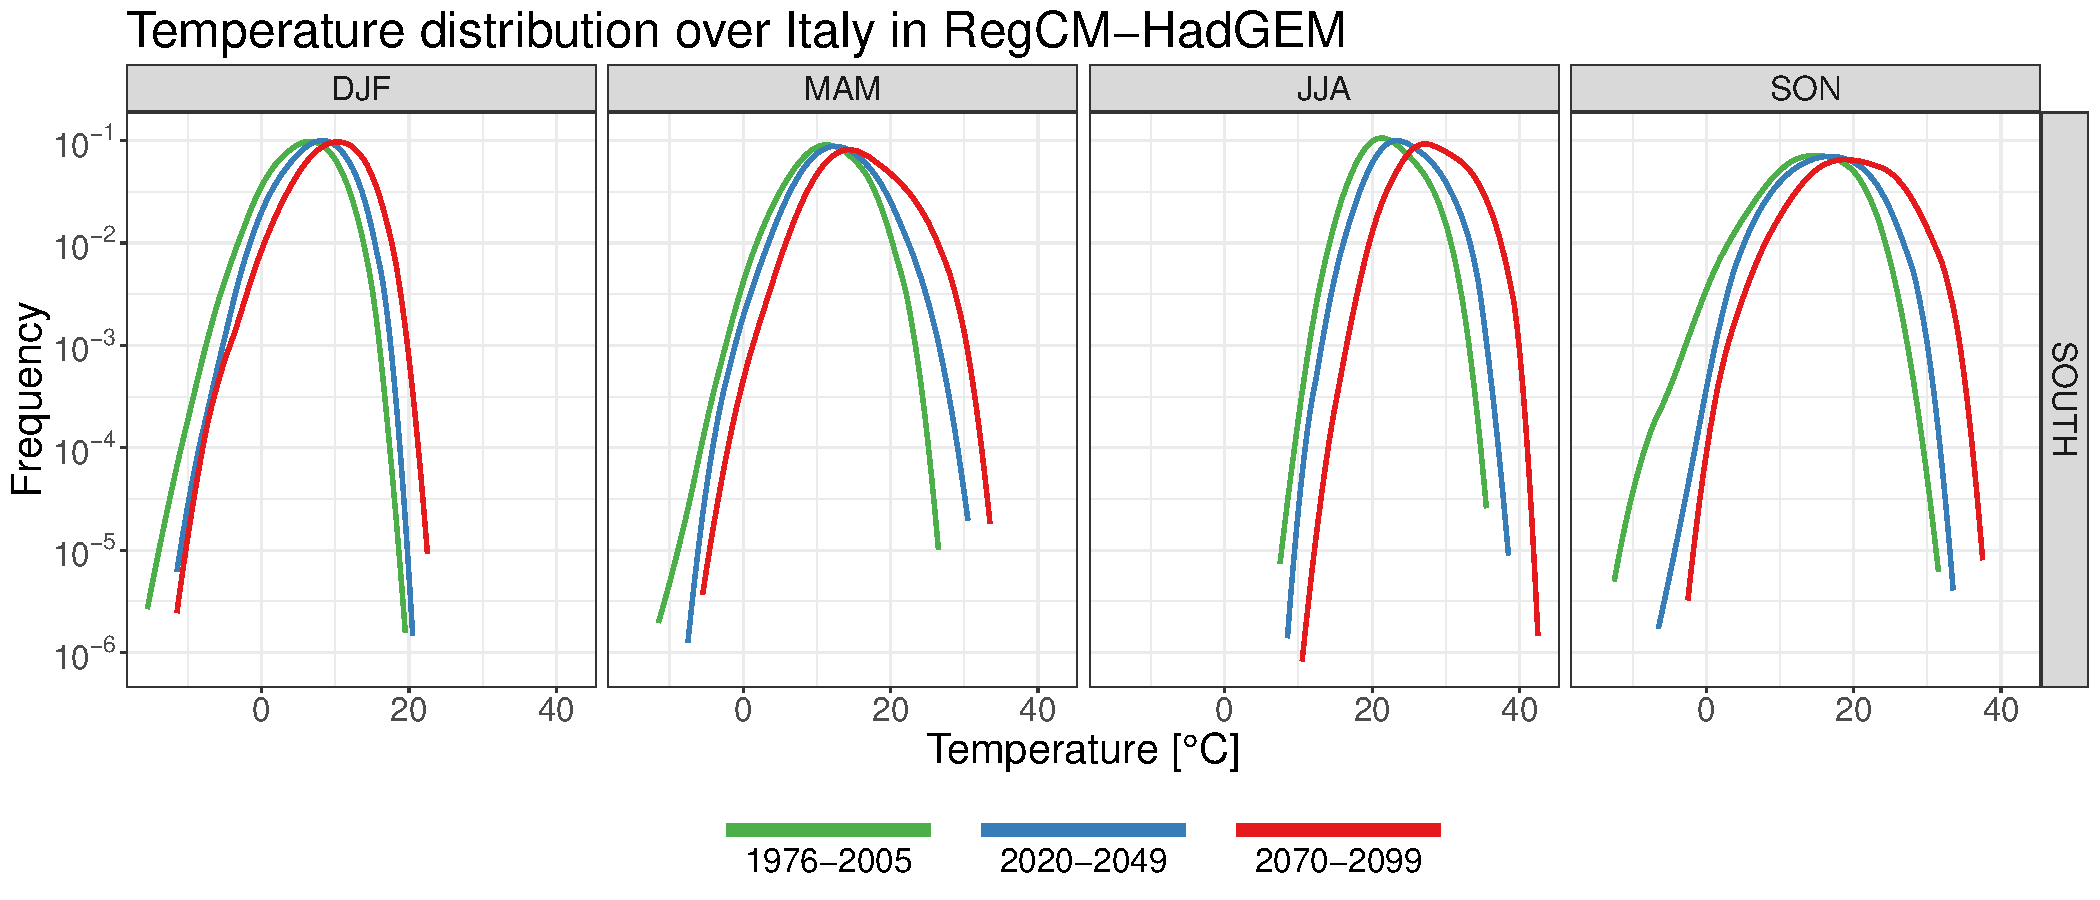
\includegraphics[width=\textwidth]{figures/change_rcm/tas/pdf_SOUTH_lines}
    \end{subfigure}\\
    \begin{subfigure}{0.8\textwidth}
        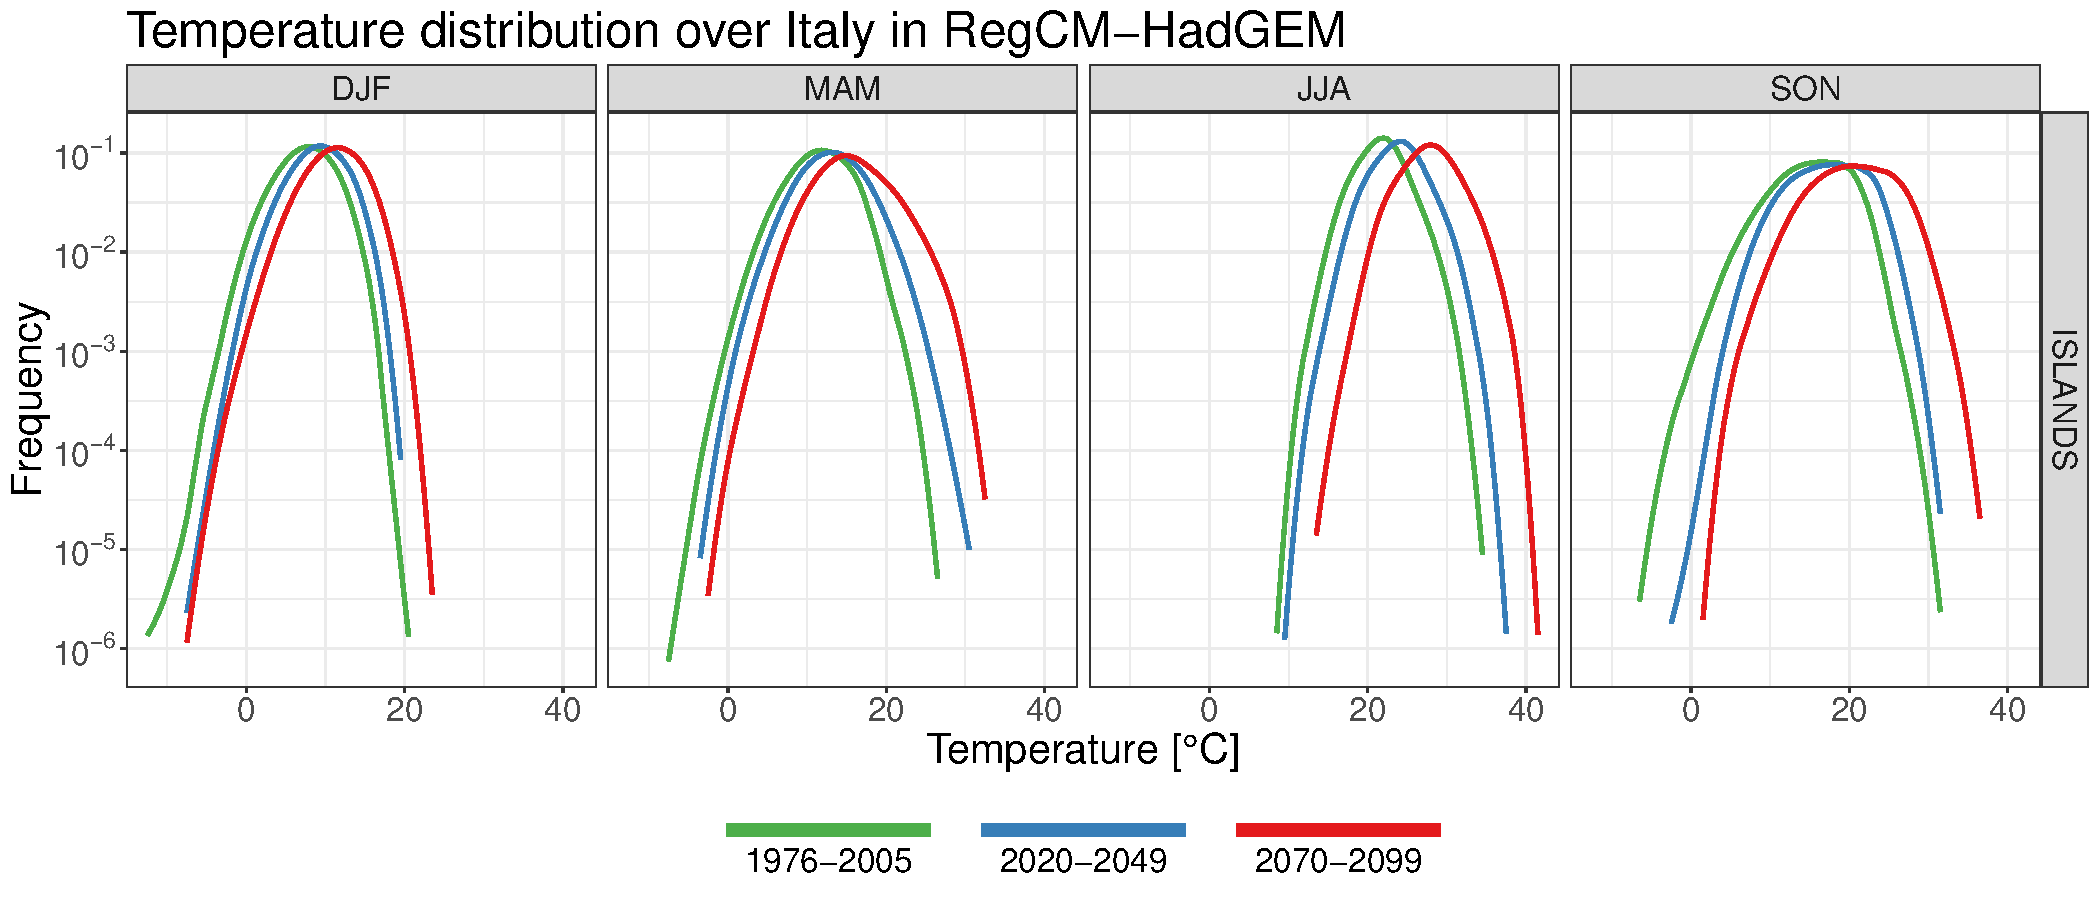
\includegraphics[width=\textwidth]{figures/change_rcm/tas/pdf_ISLANDS_lines}
    \end{subfigure}
    \decoRule
    \caption[Validation of temperature PDFs]{
        Daily seasonal temperature Probability Density Functions for the RegCM (HadGEM) simulation, across the three timeslices. The four rows represent macroregions, the four columns the seasons.
    }\label{fig:change_rcm_tas_pdf}
\end{figure}
